% !TeX program = xelatex
\documentclass[a4paper,10pt]{article}

% ============================================================================
% សន្លឹកកិច្ចការសិស្ស ស-ខ្មៅ (Student Guided-Inquiry Worksheet - Grade 8 ALG52)
% បរិបទ៖ ថ្នាក់រៀនគ្មានស្លាយ LCD – ១.៤-១.៦ ប្រមាណវិធីបូក ដក គុណ និងចែកឯកធា (២ ទំព័រ A4)
% ============================================================================
\usepackage[a4paper, left=0.90cm, right=0.90cm, top=0.75cm, bottom=0.85cm, footskip=0.45cm]{geometry}
\usepackage{amsmath, amssymb}
\usepackage{unicode-math}
\usepackage{fontspec}
\usepackage{array, colortbl}
\usepackage[table]{xcolor}
\usepackage{enumitem}
\usepackage{pifont}
\usepackage{fancyhdr}
\usepackage{lastpage}
\usepackage{tikz}
\usepackage[most]{tcolorbox}
\usetikzlibrary{calc, arrows.meta, positioning, babel}

\makeatletter
\let\@expl@@@mark@update@singlecol@structures@@\relax
\makeatother

\providecommand{\NGSFindFonts}{%
  \IfFileExists{C:/Windows/Fonts/cambria.ttc}{%
    \def\NGSSysPath{C:/Windows/Fonts/}%
    \def\NGSUserPath{C:/Users/KIT/AppData/Local/Microsoft/Windows/Fonts/}%
  }{%
    \IfFileExists{./fonts/KhmerOSsiemreap.ttf}{\def\NGSSysPath{./fonts/}\def\NGSUserPath{./fonts/}}{%
    \IfFileExists{../fonts/KhmerOSsiemreap.ttf}{\def\NGSSysPath{../fonts/}\def\NGSUserPath{../fonts/}}{%
    \IfFileExists{../../fonts/KhmerOSsiemreap.ttf}{\def\NGSSysPath{../../fonts/}\def\NGSUserPath{../../fonts/}}{%
    \IfFileExists{../../../fonts/KhmerOSsiemreap.ttf}{\def\NGSSysPath{../../../fonts/}\def\NGSUserPath{../../../fonts/}}{%
    \IfFileExists{../../../../fonts/KhmerOSsiemreap.ttf}{\def\NGSSysPath{../../../../fonts/}\def\NGSUserPath{../../../../fonts/}}{%
    \IfFileExists{../../../../../fonts/KhmerOSsiemreap.ttf}{\def\NGSSysPath{../../../../../fonts/}\def\NGSUserPath{../../../../../fonts/}}{%
    \IfFileExists{../../../../../../fonts/KhmerOSsiemreap.ttf}{\def\NGSSysPath{../../../../../../fonts/}\def\NGSUserPath{../../../../../../fonts/}}{%
      \def\NGSSysPath{../../../../../../../fonts/}\def\NGSUserPath{../../../../../../../fonts/}%
    }}}}}}}%
  }%
}
\NGSFindFonts

\setmathfont[Path={\NGSSysPath}, FontIndex=1, Scale=1.02]{cambria.ttc}
\defaultfontfeatures{Ligatures=TeX}

\setmainfont[
  Path={\NGSUserPath},
  Extension=.ttf,
  Script=Khmer,
  BoldFont={KhmerOSsiemreap},
  BoldFeatures={FakeBold=1.8},
  ItalicFont={KhmerOSsiemreap},
  ItalicFeatures={FakeSlant=0.25},
  BoldItalicFont={KhmerOSsiemreap},
  BoldItalicFeatures={FakeBold=1.8, FakeSlant=0.25}
]{KhmerOSsiemreap}

\newfontfamily\muol[Path={\NGSUserPath}, Extension=.ttf, Script=Khmer]{KhmerOSmuollight}
\newfontfamily\TimesEn[Path={\NGSSysPath}, Extension=.ttf, BoldFont={timesbd}, ItalicFont={timesi}, BoldItalicFont={timesbi}]{times}

\XeTeXlinebreaklocale "km"
\XeTeXlinebreakskip = 0pt plus 1pt minus 0.1pt

\definecolor{panelgray}{gray}{0.94}
\definecolor{headgray}{gray}{0.86}

\pagestyle{fancy}
\fancyhf{}
\renewcommand{\headrulewidth}{0pt}
\fancyfoot[L]{\fontsize{8pt}{10pt}\selectfont អនុវិទ្យាល័យព្រះក្រសាំង \en{|} គណិតវិទ្យា ថ្នាក់ទី៨ \en{|} មេរៀនទី៥ (១.៤--១.៦ ប្រមាណវិធីបូក ដក គុណ និងចែកឯកធា)}
\fancyfoot[R]{\fontsize{8.2pt}{10pt}\selectfont ទំព័រ \en{\thepage\ / \pageref{LastPage}}}

\setlength{\parindent}{0pt}
\setlength{\parskip}{0pt}
\setlength{\tabcolsep}{4pt}

\newcommand{\en}[1]{{\TimesEn #1}}
\newcommand{\enbf}[1]{{\TimesEn\textbf{#1}}}
\newcommand{\unit}[1]{\,\text{\en{#1}}}
\newcommand{\cnum}[1]{{\fontsize{10pt}{12pt}\selectfont\ding{\numexpr171+#1\relax}}}
\newcommand{\chk}{\tikz[baseline=-0.15ex]\draw[black, line width=0.8pt] (0,0) rectangle (0.25cm,0.25cm);}
\newcommand{\dotline}[1]{\makebox[#1]{\dotfill}}

\newcolumntype{L}[1]{>{\raggedright\arraybackslash}p{#1}}
\newcolumntype{C}[1]{>{\centering\arraybackslash}p{#1}}

\newcommand{\secbar}[2]{%
  \vspace{3pt}
  \noindent\colorbox{headgray}{\parbox{\dimexpr\linewidth-2\fboxsep\relax}{%
    \vspace{1.5pt}{\muol\fontsize{9.5pt}{13.5pt}\selectfont #1}\hfill{\fontsize{8.5pt}{12pt}\selectfont\textbf{#2}}\vspace{1.5pt}%
  }}\par\vspace{3pt}
}

\begin{document}
\fontsize{9.5pt}{14.2pt}\selectfont

% ============================================================================
% ទំព័រទី១៖ ក្បាលសន្លឹកកិច្ចការ + E1 + E2 + E3
% ============================================================================
\begin{tcolorbox}[enhanced, sharp corners, colback=white, colframe=black, boxrule=1.0pt, top=4pt, bottom=4pt, left=6pt, right=6pt]
  \begin{center}
    {\muol\fontsize{10.5pt}{15pt}\selectfont សន្លឹកកិច្ចការសិស្ស — មេរៀនទី៥៖ កន្សោមពីជគណិត \enbf{(}១.៤--១.៦ ប្រមាណវិធីលើឯកធា\enbf{)}}\\[2pt]
    {\footnotesize សៀវភៅសិក្សាគោលថ្នាក់ទី៨ ទំព័រ ៥៣--៥៦ \en{|} ប្រៀបធៀបគំរូបន្ទះផ្ទៃក្រឡា និងគំរូចតុកោណកែង (គ្មានស្លាយ \en{LCD})}
  \end{center}
  \vspace{2pt}
  \hrule height 0.5pt
  \vspace{4pt}
  ឈ្មោះសិស្ស៖ \dotline{5.3cm} ថ្នាក់៖ \dotline{2.0cm} ដៃគូទី៖ \dotline{2.0cm} កាលបរិច្ឆេទ៖ \dotline{3.3cm}
\end{tcolorbox}

% -------------------- ផ្នែកទី១៖ E1 ENGAGE --------------------
\secbar{ផ្នែកទី១ ៖ បេសកកម្មភ្ជាប់បញ្ហា \enbf{(E1 — Engage)} — អន្ទាក់និទស្សន្តពេលបូក ទល់នឹងពេលគុណ!}{\en{3} នាទី (ទស្សន៍ទាយមុនរៀន)}

\begin{tcolorbox}[enhanced, sharp corners, colback=panelgray, colframe=black, boxrule=0.8pt, top=3.5pt, bottom=3.5pt, left=6pt, right=6pt]
  សិស្សពីរនាក់ប្រកែកគ្នាអំពីផលបូក $2xy + 5xy$ និងផ្ទៃក្រឡាសួនច្បារ $(5x)(2x)$ ។ ចូរគូសធីកការទស្សន៍ទាយរបស់អ្នកមុនរៀន៖\\[2pt]
  ១) តើ $2xy + 5xy$ ស្មើប៉ុន្មាន? \quad \chk\ មតិសុខ៖ $7x^2y^2$ (បូកទាំងនិទស្សន្ត) \qquad \chk\ មតិធីតា៖ $7xy$ (រក្សាផ្នែកអថេរដដែល)\\[2pt]
  ២) តើផ្ទៃសួនច្បារបណ្ដោយ $5x$ និងទទឹង $2x$ ស្មើប៉ុន្មាន? \quad \chk\ $10x$ \qquad \chk\ $10x^2$ \qquad \chk\ $7x^2$
\end{tcolorbox}

% -------------------- ផ្នែកទី២៖ E2 EXPLORE --------------------
\secbar{ផ្នែកទី២ ៖ រុករកវិធានបូក-ដក គុណ និងចែកឯកធា \enbf{(E2 — Explore)}}{\en{11} នាទី (ពិភាក្សាដៃគូ)}

\textbf{ក. សកម្មភាពទី១ (បូក និងដកឯកធាដូចគ្នាតាមផ្ទៃបន្ទះចតុកោណកែង ទំ.៥៣)៖}\par\vspace{2pt}
\begin{minipage}[c]{12.6cm}
  \begin{enumerate}[label=\arabic*., leftmargin=0.5cm, itemsep=3.5pt, topsep=2pt]
    \item បន្ទះចតុកោណកែង ៣ មានកម្ពស់ $b$ និងទទឹង $1, 2, 3$ ដាក់តម្រៀបជាប់គ្នា (រូបស្ដាំ)៖\\
    ទទឹងសរុបស្មើ $1 + 2 + 3 = \dotline{1.2cm}$ ហើយកម្ពស់នៅតែស្មើ $\dotline{1.2cm}$ ដដែល ។\\
    ដូចនេះ៖ $b + 2b + 3b = (1 + 2 + 3)b = \dotline{1.8cm}$ \quad (តើក្លាយជា $6b^3$ ដែរឬទេ? \chk\ ទេ \;\chk\ មែន)
    \item ចំពោះផលដក (ទំ.៥៣)៖ យកបន្ទះ $5x$ ដកចេញ $2x$ គេបាន $5x - 2x = (5 - \dotline{0.9cm})x = \dotline{1.6cm}$ ។
    \item ចុះបើបូកឯកធាដូចគ្នាដែលមានមេគុណផ្ទុយគ្នា៖ $\dfrac{1}{2}xy + \left(-\dfrac{1}{2}xy\right) = \dotline{1.8cm}$ ។
  \end{enumerate}
\end{minipage}\hfill
\begin{minipage}[c]{5.8cm}
  \centering
  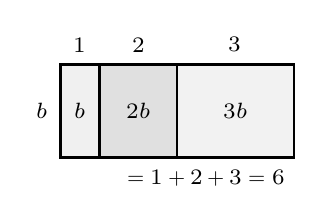
\begin{tikzpicture}[scale=0.76, every node/.style={font=\footnotesize, text=black}]
    \draw[black, line width=0.9pt, fill=gray!12] (0,0) rectangle (0.65,1.55);
    \draw[black, line width=0.9pt, fill=gray!24] (0.65,0) rectangle (1.95,1.55);
    \draw[black, line width=0.9pt, fill=gray!10] (1.95,0) rectangle (3.90,1.55);
    \node[left=1pt] at (0,0.78) {$b$};
    \node[above=1pt] at (0.32,1.55) {$1$};
    \node[above=1pt] at (1.30,1.55) {$2$};
    \node[above=1pt] at (2.92,1.55) {$3$};
    \node at (0.32,0.78) {$b$};
    \node at (1.30,0.78) {$2b$};
    \node at (2.92,0.78) {$3b$};
    \node[below=1pt] at (1.95,0) {ទទឹងសរុប $= 1+2+3=6$};
  \end{tikzpicture}
\end{minipage}

\vspace{5pt}
\textbf{ខ. សកម្មភាពទី២ (គុណឯកធាតាមផ្ទៃសួនច្បារ ទំ.៥៤ និងចែកឯកធាតាមស្រះទឹក ទំ.៥៥)៖}\par\vspace{2pt}
\begin{minipage}[c]{12.6cm}
  \begin{enumerate}[label=\arabic*., leftmargin=0.5cm, itemsep=3.5pt, topsep=1pt]
    \item \textbf{សួនច្បាររាងចតុកោណកែង} មានបណ្ដោយ $5x$ និងទទឹង $2x$ ៖\\
    ផ្ទៃក្រឡា $= (5x)(2x) = (5 \times \dotline{0.9cm})(x \times \dotline{0.9cm}) = \dotline{1.7cm}$ ។\\
    អនុវត្ត៖ $(4x^2yc^4)(3xy^3c) = (4\times 3)(x^{2+\Box})(y^{1+\Box})(c^{4+\Box}) = \dotline{2.4cm}$ ។
    \item \textbf{ស្រះទឹករាងចតុកោណកែង} មានផ្ទៃក្រឡា $16xy^2$ និងទទឹង $4y$ ៖\\
    បណ្ដោយ $= \dfrac{16xy^2}{4y} = \dfrac{16}{4} \cdot x \cdot y^{2-\Box} = \dotline{1.8cm}$ ។\\
    អនុវត្ត៖ $(8x^4y^5) \div (16x^2y^3) = \dfrac{8}{16}\,x^{4-\Box}\,y^{5-\Box} = \dotline{2.3cm}$ ($\frac{8}{16}=\frac{1}{\Box}$) ។
  \end{enumerate}
\end{minipage}\hfill
\begin{minipage}[c]{5.8cm}
  \centering
  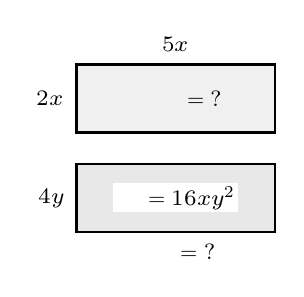
\begin{tikzpicture}[scale=0.72, every node/.style={font=\footnotesize, text=black}]
    \draw[black, line width=0.85pt, fill=gray!12] (0,1.75) rectangle (3.5,2.95);
    \node[left=1pt] at (0,2.35) {$2x$};
    \node[above=1pt] at (1.75,2.95) {$5x$};
    \node at (1.75,2.35) {សួនច្បារ $= \text{?}$};
    \draw[black, line width=0.85pt, fill=gray!18] (0,0) rectangle (3.5,1.20);
    \node[left=1pt] at (0,0.60) {$4y$};
    \node[below=1pt] at (1.75,0) {បណ្ដោយ $= \text{?}$};
    \node[fill=white, inner sep=1pt] at (1.75,0.60) {ផ្ទៃ $= 16xy^2$};
  \end{tikzpicture}
\end{minipage}

% -------------------- ផ្នែកទី៣៖ E3 EXPLAIN --------------------
\secbar{ផ្នែកទី៣ ៖ តារាងសង្ខេបវិធានប្រមាណវិធី និងធនាគារហេតុផល \enbf{(E3 — Explain)}}{\en{6} នាទី (កត់ត្រាខ្លឹមសារគោល)}

{\renewcommand{\arraystretch}{1.48}
\begin{tabular}{|L{4.2cm}|L{8.8cm}|L{4.8cm}|}
\hline
\cellcolor{headgray}\textbf{ប្រមាណវិធីលើឯកធា} & \cellcolor{headgray}\textbf{វិធានគណនា (មេគុណ និងនិទស្សន្ត)} & \cellcolor{headgray}\textbf{គំរូសម្គាល់រហ័ស} \\
\hline
\cnum{1} \textbf{បូក / ដក} (ទំ.៥៤)\newline \textit{(តែឯកធាដូចគ្នាប៉ុណ្ណោះ!)} & បូក ឬដកតែផ្នែក \dotline{2.3cm} រួចរក្សាផ្នែក \dotline{2.3cm} ឱ្យនៅដដែល (\textbf{ហាម}បូកនិទស្សន្ត!) & $2xy + 5xy = \dotline{2.2cm}$ \\
\hline
\cnum{2} \textbf{គុណឯកធា} (ទំ.៥៤) & គុណមេគុណនឹង \dotline{2.2cm} ហើយ \textbf{\dotline{1.8cm} និទស្សន្ត} តាមអថេរដូចគ្នា ($a^m\cdot a^n = a^{m+n}$) & $(5x)(2x) = \dotline{2.2cm}$ \\
\hline
\cnum{3} \textbf{ចែកឯកធា} (ទំ.៥៥) & ចែកមេគុណនឹង \dotline{2.2cm} ហើយ \textbf{\dotline{1.8cm} និទស្សន្ត} តាមអថេរដូចគ្នា ($\frac{a^m}{a^n} = a^{m-n}$; \cnum{4} $\frac{y}{y}=1$) & $\dfrac{16xy^2}{4y} = \dotline{2.2cm}$ \\
\hline
\end{tabular}}

\vspace{5pt}
\begin{tcolorbox}[enhanced, sharp corners, colback=panelgray, colframe=black, boxrule=0.8pt, top=3.5pt, bottom=3.5pt, left=6pt, right=6pt]
  \ding{43}\; \textbf{ប្រអប់ប្រុងប្រយ័ត្នកំហុសញឹកញាប់៖} ឯកធាមិនដូចគ្នា \textbf{អាចគុណ ឬចែកគ្នាបាន} (ឧ. $(2x^2)(3x) = 6x^3$) ប៉ុន្តែ \textbf{ហាមបូក ឬដកបញ្ចូលគ្នាដាច់ខាត} (ឧ. $2x^2 + 3x$ ត្រូវរក្សាទុកជា $2x^2 + 3x$ ដដែល មិនស្មើ $5x^3$ ឡើយ!) ។
\end{tcolorbox}

\newpage
% ============================================================================
% ទំព័រទី២៖ E4 (លំហាត់គំរូ ទំ.៥៤-៥៦) + E5 (ប្រតិបត្តិ + Exit Check) + កិច្ចការផ្ទះ
% ============================================================================

% -------------------- ផ្នែកទី៤៖ E4 ELABORATE --------------------
\secbar{ផ្នែកទី៤ ៖ អនុវត្តលំហាត់គំរូតាមសៀវភៅគោល \enbf{(E4 — Elaborate)}}{\en{10} នាទី (បំពេញតាមគំរូ)}

\textbf{១. លំហាត់គំរូបូក-ដកឯកធាដូចគ្នា (ទំ.៥៤) និងផ្ទៃប្លង់ភូមិគ្រឹះ (ទំ.៥៥)៖}
\begin{itemize}[leftmargin=0.5cm, itemsep=3pt, topsep=2pt]
  \item \textbf{គំរូ ខ (ទំ.៥៤ — ប្រយ័ត្នមេគុណលាក់មុខ $1$)៖} $3ab^2 + 7ab^2 + ab^2 = (3 + 7 + \dotline{0.9cm})ab^2 = \dotline{2.3cm}$ ។
  \item \textbf{គំរូ គ (ទំ.៥៤ — ប្រយ័ត្នសញ្ញាដកបន្តបន្ទាប់)៖} $8x^2y^3z - 3x^2y^3z - 7x^2y^3z = (8 - 3 - 7)x^2y^3z = \dotline{2.6cm}$ ។
  \item \textbf{ផ្ទៃក្រឡាប្លង់ភូមិគ្រឹះ (ទំ.៥៥)៖} បណ្ដោយ $18a$ និងទទឹង $12a$ $\implies A = (18a)(12a) = (18\times 12)(a\times a) = \dotline{2.4cm}$ ឯកតាផ្ទៃ ។
\end{itemize}

\vspace{2pt}
\textbf{២. លំហាត់គំរូវិធីចែកឯកធា (សៀវភៅគោល ទំ.៥៦)៖}
\begin{itemize}[leftmargin=0.5cm, itemsep=3pt, topsep=2pt]
  \item ក) $(5xy^3) \div (xy) = \dfrac{5xy^3}{1xy} = 5\,x^{1-1}\,y^{3-1} = \dotline{2.4cm}$ \qquad
        ខ) $\dfrac{18xyz^3}{9yz^2} = \dfrac{18}{9}\cdot x \cdot \dfrac{y}{y} \cdot z^{3-2} = \dotline{2.4cm}$
  \item គ) $1a^2b^3 \div 2ab = \dfrac{1a^2b^3}{2ab} = \dotline{2.8cm}$ \qquad\textit{(ទុកមេគុណជាប្រភាគ $\dfrac{1}{2}$)}
\end{itemize}

\vspace{2pt}
$\bullet$ \textbf{សំណួរឆ្លុះបញ្ចាំង (\en{Looking Back})៖} តើយើងអាចបូកបង្រួម $3x^2y + 5xy^2$ ឱ្យទៅជា $8x^3y^3$ បានដែរឬទេ? ព្រោះអ្វី?\\
ចម្លើយ៖ \chk\ បាន \quad \chk\ មិនបានទេ ព្រោះ $3x^2y$ និង $5xy^2$ \dotline{8.8cm} ។

% -------------------- ផ្នែកទី៥៖ E5 EVALUATE --------------------
\secbar{ផ្នែកទី៥ ៖ ហ្វឹកហាត់ «ប្រតិបត្តិ» និងតេស្តរហ័ស \enbf{(E5 — Evaluate)}}{\en{10} នាទី (ធ្វើដោយខ្លួនឯង រួចប្ដូរផ្ទៀង)}

{\renewcommand{\arraystretch}{1.42}
\begin{tabular}{|L{9.1cm}|L{9.1cm}|}
\hline
\multicolumn{2}{|l|}{\cellcolor{headgray}\textbf{១. ប្រតិបត្តិបូក-ដកឯកធាដូចគ្នា (សៀវភៅគោល ទំ.៥៤)}} \\
\hline
ក. $5x^2y - 3x^2y = \dotline{4.8cm}$ & ខ. $3ac^2b^3 + (-4ac^2b^3) + 7ac^2b^3 = \dotline{3.0cm}$ \\
\hline
\multicolumn{2}{|l|}{ច. $\dfrac{1}{2}ac^2b^3 + \left(-\dfrac{1}{2}ac^2b^3\right) + 7ac^2b^3 = \dotline{7.5cm}$} \\
\hline
\multicolumn{2}{|l|}{\cellcolor{headgray}\textbf{២. ប្រតិបត្តិគុណឯកធា (សៀវភៅគោល ទំ.៥៥)}} \\
\hline
ក. $(5xy^3)(x^2y) = \dotline{4.8cm}$ & គ. $\left(\dfrac{1}{2}ab^3\right)(3a^2b^2) = \dotline{4.2cm}$ \\
\hline
\multicolumn{2}{|l|}{ខ. $(ab^2c^3)(-4ac^2b)(acb) = \dotline{8.5cm}$} \\
\hline
\multicolumn{2}{|l|}{\cellcolor{headgray}\textbf{៣. ប្រតិបត្តិចែកឯកធា (សៀវភៅគោល ទំ.៥៦)}} \\
\hline
ក. $x^{3n} \div x^{2n} = x^{3n - \dots\dots} = \dotline{3.5cm}$ & ឃ. $\dfrac{xyz^3}{yz^2} = \dotline{4.8cm}$ \\
\hline
\multicolumn{2}{|l|}{ច. $81z^{12}b^3 \div 3z^{12}b = \dotline{8.8cm}$} \\
\hline
\end{tabular}}

\vspace{4pt}
\begin{tcolorbox}[enhanced, sharp corners, colback=panelgray, colframe=black, boxrule=0.85pt, top=3pt, bottom=3pt, left=6pt, right=6pt]
  \textbf{៤. បិទបេសកកម្ម \en{E1} និងតេស្តរហ័ស (\en{Exit Check — 60} វិនាទី)៖}\\[2pt]
  $\bullet$ \textbf{ចម្លើយបេសកកម្ម \en{E1}៖} $2xy + 5xy = \dotline{2.0cm}$ ចំណែក $(5x)(2x) = \dotline{2.0cm}$ ។\\[2pt]
  $\bullet$ \textbf{សំណួរតេស្តរហ័ស៖} តើគូប្រមាណវិធីណាមួយខាងក្រោមគណនាបាន \textbf{ត្រឹមត្រូវទាំងពីរ}? (គូសរង្វង់ជម្រើសតែមួយ)៖\\[2pt]
  \hspace*{0.2cm}\enbf{A.}\; $4a^2b + 2a^2b = 6a^4b^2$ និង $(4a^2b)(2a^2b) = 8a^4b^2$ \qquad
  \enbf{B.}\; $4a^2b + 2a^2b = 6a^2b$ និង $(4a^2b)(2a^2b) = 8a^4b^2$\\[1.5pt]
  \hspace*{0.2cm}\enbf{C.}\; $4a^2b + 2a^2b = 6a^2b$ និង $(4a^2b)(2a^2b) = 6a^4b^2$ \qquad
  \enbf{D.}\; $4a^2b + 2a^2b = 6a^2b$ និង $(4a^2b)(2a^2b) = 6a^2b$
\end{tcolorbox}

% -------------------- ផ្នែកទី៦៖ កិច្ចការផ្ទះ --------------------
\secbar{ផ្នែកទី៦ ៖ ប័ណ្ណកិច្ចការផ្ទះ \enbf{(Homework)} និងការអានជាមុន}{សៀវភៅគោល ទំ.៥៥--៥៦ និង ៧២--៧៣}

\begin{tcolorbox}[enhanced, sharp corners, colback=white, colframe=black, boxrule=0.8pt, borderline={0.6pt}{2pt}{dashed}, top=3pt, bottom=3pt, left=6pt, right=6pt]
  \textbf{១. លំហាត់ទី៣ ក--ខ (ទំ.៧២) និងទី៥ ក (ទំ.៧៣)៖} គណនាកន្សោមខាងក្រោមក្នុងសៀវភៅកិច្ចការផ្ទះ៖
  \[ \text{ក)}\; 3x^2 + 7x^2 - 5x^2 \qquad\quad \text{ខ)}\; \frac{3}{2}x^4y^4t + 2x^4y^4t - x^4y^2t \;\text{(ពិនិត្យផ្នែកអថេរតួទី៣!)} \qquad\quad \text{៥ក)}\; 3x^2y^2 + 2x^2y^2 \]
  \textbf{២. ប្រតិបត្តិគុណ និងចែកបន្ថែម (ទំ.៥៥--៥៦)៖} គណនា៖ $(-4y^3c^2b^3)(8yc^2b)$ \quad និង \quad $\dfrac{ax^7b^5}{ax^5b^3}$ ។\\[1.5pt]
  $\bullet$ \textbf{អានជាមុន៖} ចំណុច \textbf{២.១--២.៣ សញ្ញាណពហុធា ដឺក្រេ និងវិធីបូក-ដកពហុធា} (សៀវភៅគោល ទំព័រ ៥៦--៥៩) ។
\end{tcolorbox}

\end{document}
